%!TEX root = ../problems.tex
\begin{task}
	Найти и нарисовать амплитудно-частотную характеристику (АЧХ) для цепи, изображённой на рисунке. 
\end{task}
% \begin{figure}[h!]
% 	\centering
% 	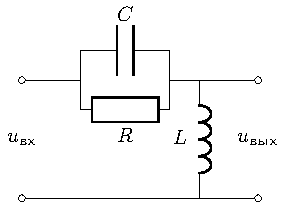
\includegraphics[scale=2]{chem/task7}
% 	\caption{}
% 	\label{fig:7}
% \end{figure}
\vspace{-1em}
\begin{figure}[ht]
  \centering
  \begin{subfigure}[b]{0.5\linewidth}
    \centering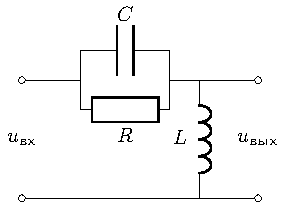
\includegraphics[scale=1.8]{chem/task7}
    \vspace{0.15em}
    % \caption{\label{fig:fig2}}
  \end{subfigure}%
  \begin{subfigure}[b]{0.5\linewidth}
    \centering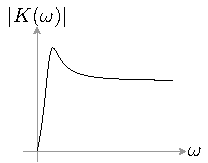
\includegraphics[scale=1.8]{ris/task7_out2}
    % \caption{\label{fig:fig1}}
  \end{subfigure}%
  \caption{Цепь и найденная её АЧХ}
\end{figure}

Последовательно найдем импеданс входной цепи $Z$: сначала найдем эквивалентный импеданс  $Z_\text{экв}$ параллельной $RC$-цепочки, затем суммарный импеданс $Z=Z_\text{экв}+j\omega L$ последовательно соединенных $RC$-цепочки и катушки индуктивности $L$.
\begin{gather*}
	\hat{Z}_\text{экв}=\frac{\hat{Z}_R \cdot \hat{Z}_C}{\hat{Z}_R + \hat{Z}_C}=\frac{R \cdot \frac{1}{j\omega C}}{R + \frac{1}{j\omega C}}=\frac{R}{1+j\omega CR}=\frac{R(1-j\omega CR)}{1+(\omega CR)^2}=\frac{R-j\omega CR^2}{1+(\omega CR)^2}
\end{gather*}
Коэффициент передачи будем искать по определению, как отношение выходного сигнала к входному, считая, что в цепи течет ток $I$:
\begin{gather*}
	\hat{K}=\frac{\hat{u}_\out}{\hat{u}_\in}=\frac{\hat{I} \cdot \hat{Z}_{L}}{\hat{I} \cdot (\hat{Z}_{L}+\hat{Z}_{\text{экв}})}=\frac{\hat{Z}_{L}}{(\hat{Z}_{L}+\hat{Z}_{\text{экв}})}=\frac{j\omega L}{j\omega L+\frac{R}{1+j\omega CR}}=\\=\frac{j\omega L(1+j\omega CR)}{R+j\omega L(1+j\omega CR)}=\frac{j\omega L-\omega^2LCR}{R-\omega^2LCR+j\omega L}
\end{gather*}
Отсюда окончательно получаем выражение для модуля коэффициента передачи:
\begin{gather*}
	K=|\hat{K}(\omega)|=\frac{\sqrt{(\omega^2LRC)^2+(\omega L)^2}}{\sqrt(R-\omega^2LRC)^2+(\omega L)^2}=\frac{\sqrt{(RLC)^2+\frac{L^2}{\omega^2}}}{\sqrt{(\frac{R}{\omega^2}-RLC)^2+\frac{L^2}{\omega^2}}}
\end{gather*}
